%% Digital Systems
%% Introduction
\def\FileDate{98/11/04}
\def\FileVersion{1.0}
% ----------------------------------------------------------------
% Notes pages *********************************************************
% ----------------------------------------------------------------

\begin{slide}\label{slide:l7s1}
\heading{Introduction}
\begin{itemize}
\item Digital systems are important in modern technology because they
  are used extensively to implement designs that previously used
  analogue (continuous) technology.
\item The concepts developed for continuous systems
  are all applicable to digital systems.
\item This introduction commences with digital signals, continues with
  digital systems, and ends with an overview of how analogue systems
  may be converted to digital systems.
\end{itemize}
\end{slide}

\begin{slide}\label{slide:l7s1a}
\heading{Analogue v Digital}
\begin{itemize}
\item The real world we inhabit is analogue. We process analogue
  signals: e.g. vision and sound. Physical systems are analogue
  systems of force, velocity, current, voltage, temperature pressure,
  etc.
\item Advances in electronics means that more and more of the storage,
  distribution and processing of signals is actually done using
  digital technology.
\item There have to be methods of converting analogue to digital (e.g.
  recording of sound) and digital to analogue (e.g. signals delivered
  by loudspeakers).
\item We need to be able to model the signals, their conversion and
  the systems that process them.
\end{itemize}
\end{slide}

\section*{Samplers and Discrete-Time Physical Systems}

As hinted in the introduction, we need to convert analogue signals to
digital sigals before the digtal signal can be stored, distibuted and
manipulated by a digital system. At the point of delivery, we need to
convert the signal back into digital form. In this section we
introduce the signal conversion devices and give an example of one
commonly seen digital system.

\subsection*{Analogue to Digital Converter}

We begin by describing the \emph{digital to analogue converter} (D/A
or DAC), since this device is usually also a component of the
\emph{analogue to digital compensator} (A/D or ADC). We assume that
the DAC receives a digital signal, in the form of a binary number,
every $T$ seconds (usually from a digital computer, microcontroller or
a digital signal processor). The DAC converts the binary number to a
constant voltage equal to the value of that number, and outputs this
voltage until the next number arrives and the DAC input. The block
diagram of the DAC and a typical response is shown in
\sref{slide:DAC}.

\begin{slide}\label{slide:DAC}
\heading{Digital to Analogue Converter (D/A or DAC)}
\begin{center}
  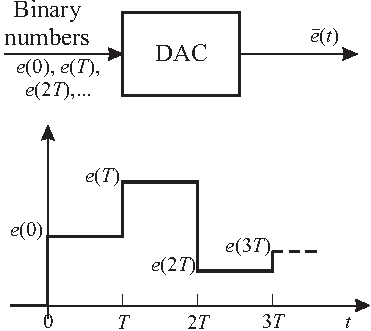
\includegraphics{pictures/DAC.pdf}
\end{center}
\end{slide}

We next describe a comparitor, which is also a component of the ADC. A
comparitor and its characteristics are illustrated in
\sref{slide:compare}. The input voltage $v_i(t)$ is compared with the
reference voltage $v_r(t)$.  If $v_i(t) > v_r(t)$ the comparitor
outputs logic ``1''; for example logic 1 is 5V for TTL logic.  If
$v_i(t) < v_r(t)$ the comparitor outputs logic ``0''; which is less
than 1V for TTL logic. The signal ground is normally omitted from
circuit diagrams, but all voltages are compared relative to signal
ground.

\begin{slide}\label{slide:compare}
\heading{Voltage Comparitor}
\begin{center}
  \resizebox{250pt}{!}{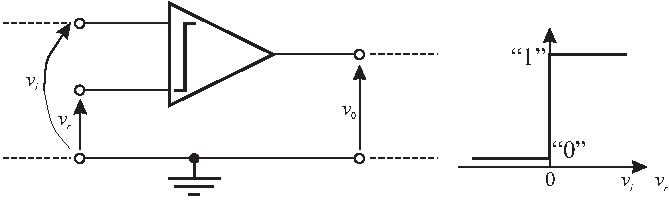
\includegraphics{pictures/comparitor.pdf}}
\end{center}
\end{slide}

Several circuits are used to implement an analogue to digital
converter. Each circuit has different characteristics. We illustate
the up-counter ADC shown in \sref{slide:ADC}. The $n$-bit counter is
reset to zero when the start-of-conversion (SOC) signal is received by
the device. The count increases by 1 with the arrival of each clock
pulse. The $n$-bit DAC converts the binary equivalent of the count to
a voltage $v_R$. 

\begin{slide}\label{slide:ADC}
\heading{Analogue to Digital Converter}
The counter ADC.
\begin{center}
  \resizebox{300pt}{!}{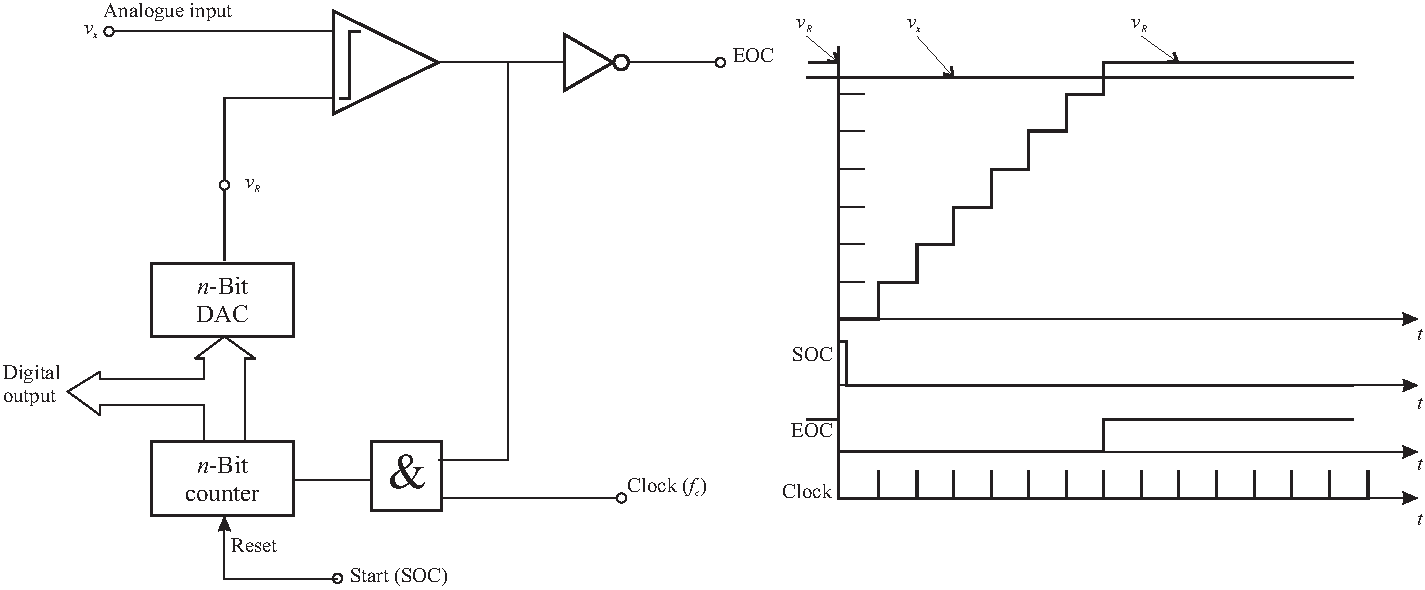
\includegraphics{pictures/ADC.pdf}}
\end{center}
\end{slide}

The analogue voltage $v_x$ to be converted is compared to $V_R$. When
$V_R$ becomes greater than $v_x$, the comparitor outputs a logic 0,
which halts the clock input through the AND gate. The
end-of-conversion (EOC) pulse then signals that the digital equivalent
to $v_x$ is ready. The counter output can then be read from the
digital output as a binary number which is approximately equal to the
analogue input.

\subsection*{Digital Systems}

Once we have the ability to convert analogue signals into binary
numbers and back, we have the ability to process the information using
computers and other digital devices. A familiar device will be the
compact disk (CD) player.

\begin{slide}\label{slide:CD1}
\heading{Compact Disk (Analogue to Digital)}
\begin{itemize}
\item Continuous time signal is filtered with an ``anti-aliasing''
  band-pass filter with bandwidth of 5 to 20,000 Hz.
\item Filtered audio signal sampled using ADC at 44,100 samples per second and
  with 14-16 bits precision. 
\item Each sample is stored, along with error
  correcting bits, as a stream of binary codes. 
\item The codes are recorded using microscopic pits etched into the surface of the CD.
\end{itemize}
\end{slide}

\begin{slide}\label{slide:CD2}
\heading{Compact Disk (Digital to Analogue)}
\begin{itemize}
\item For stereo music, two channels are sampled and stored.
\item Data is stored on a continuous track that spirals outwards from
  the centre.
\item Data is read at a constant rate (44,100 Hz) and is processed (e.g.
  error corrected and buffered for tilt control) before being
  converted, using DAC, to a signal that can be delivered to a
  loudspeaker.
\item Velocity of disk needs to be controlled so that it decreases as
  the radius of the track increases. Position and the focus of the laser used to read the data is
  also controlled.
\item Audio CD holds approx 540 MBytes of data which is enough to
  store 74 minutes of stereo music.
\end{itemize}
\end{slide}


\section*{Generation of Digital Signals}
Digital signals do not occur naturally. They are generated by
sampling continuous signals, or by digitally processing other
digital signals. Sampling is accomplished by a sampler known as an
``\emph{Analogue to Digital Converter (ADC)}''.

\begin{slide}\label{slide:l7s2a}
  \heading{Sampling and Sequences}
  \begin{itemize}
   \item Sampling -- mathematical model of the ADC
   \item Sampled signals are modelled as sequences
   \item Sequences can be shifted backwards and forwards
   \item The advance and delay operators are analogies to the derivative
     and integral operators
  \end{itemize}
\end{slide}

\begin{slide}\label{slide:l7s2}
  \heading{Sampling -- Mathematical model of the ADC}
  \center{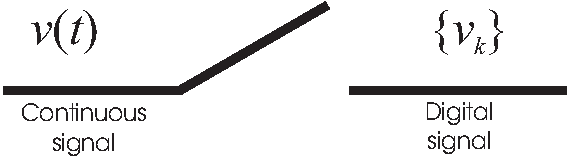
\includegraphics{pictures/sampler.pdf}}
  \begin{itemize}
   \item Quantization, introduced by converting an analogue signal to a
     binary number with a finite number of bits, will not be considered. 
  \end{itemize}
\end{slide}


The analogue to digital converter is modelled as a a switch as
shown in \sref{slide:l7s2}. 

\ifslidesonly
\begin{slide}
\heading{Modelling Sampling: Sequences}
At each sampling instant the switch is
closed for an infinitesimal time, during which the digital signal
has the same value as the continuous signal. The digital signal is
therefore a ``\emph{Sequence}'' \[\ldots\ v_{-2}\ v_{-1}\ v_{0}\
v_{1}\ v_{2}\ \ldots \] which will be denoted by
\[\left\{v_k\right\}\]
\endinput


%%% Local Variables: 
%%% mode: latex
%%% TeX-master: "notes"
%%% End: 

\end{slide}
\fi
At each sampling instant the switch is
closed for an infinitesimal time, during which the digital signal
has the same value as the continuous signal. The digital signal is
therefore a ``\emph{Sequence}'' \[\ldots\ v_{-2}\ v_{-1}\ v_{0}\
v_{1}\ v_{2}\ \ldots \] which will be denoted by
\[\left\{v_k\right\}\]
\endinput


%%% Local Variables: 
%%% mode: latex
%%% TeX-master: "notes"
%%% End: 


\ifslidesonly
\begin{slide}
\heading{Modelling Sampling: Regular Sampling}
Only regular sampling will be considered. A constant period $T$~s
between sampling instants is equivalent to a sampling frequency
$\omega_s$~rad~s$^{-1}$, where \[ T = \frac{2\pi}{\omega_s}. \]

Sampling is assumed to be synchronized to the time origin $t=0$ so
that \[ v_k = v(kT)\ \mathrm{for\ all }\ k.\]
\endinput

%%% Local Variables: 
%%% mode: latex
%%% TeX-master: "notes"
%%% End: 

\end{slide}
\fi
Only regular sampling will be considered. A constant period $T$~s
between sampling instants is equivalent to a sampling frequency
$\omega_s$~rad~s$^{-1}$, where \[ T = \frac{2\pi}{\omega_s}. \]

Sampling is assumed to be synchronized to the time origin $t=0$ so
that \[ v_k = v(kT)\ \mathrm{for\ all }\ k.\]
\endinput

%%% Local Variables: 
%%% mode: latex
%%% TeX-master: "notes"
%%% End: 


\begin{slide}\label{slide:l7s3}
\heading{Sampling: The Signals}
\center{\resizebox{250pt}{!}{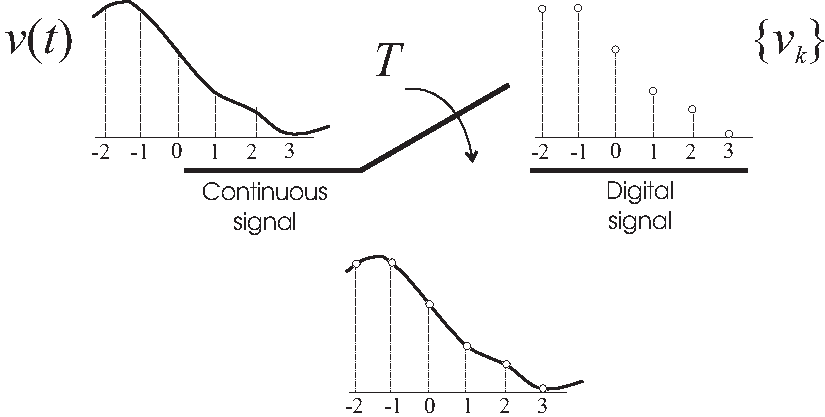
\includegraphics{pictures/sampling.pdf}}}
\end{slide}

\ifslidesonly
\begin{slide}
\heading{Indexing the Sequence}
The index $k$ denotes the current value. Digital signals will be
taken as zero prior to the time origin, in the same way as
continuous signals:
\[ v_k = v(kT) = 0\ \mathrm{for}\ k<0. \]

Except in cases where it is necessary to distinguish between them,
both the continuous signal $v(t)$ and the digital signal
$\left\{v_k\right\}$ will be denoted by $v$.
\endinput

%%% Local Variables: 
%%% mode: plain-tex
%%% TeX-master: "notes"
%%% End: 

\end{slide}
\fi
The index $k$ denotes the current value. Digital signals will be
taken as zero prior to the time origin, in the same way as
continuous signals:
\[ v_k = v(kT) = 0\ \mathrm{for}\ k<0. \]

Except in cases where it is necessary to distinguish between them,
both the continuous signal $v(t)$ and the digital signal
$\left\{v_k\right\}$ will be denoted by $v$.
\endinput

%%% Local Variables: 
%%% mode: plain-tex
%%% TeX-master: "notes"
%%% End: 


\section*{Shifting Digital Signals}
Shifting digital signals is the mechanism by which dynamic
behaviour is introduced into digital systems. The shifting
operators are comparable to differentiating and integrating
continuous signals.

\begin{slide}
  \heading{Forward Shifting a Digital Signal}\label{slide:l7s4}
\begin{itemize}

\item   The first forward shift of a digital signal $v$ is generated by
  applying the ``\emph{Advance Operator}'' $\triangle$  to give the
  advanced digital signal $\triangle v$, where \[ \triangle v = \triangle
  \{v_k\} = \{\triangle v_k\} = \{v_{k+1}\}.\]
  

\item   The signal $v$ is advanced by one value (a time advance of
  $T$). $v_0$ vanishes because $\triangle v$ is zero prior to $t=0$.


\item   Repeated operation gives the $r$-th forward shift \[
  \triangle^r v = \{v_{k+r}\}\].

\end{itemize}

\end{slide}

\begin{slide}
\heading{Advance and Derivative Operator}\label{slide:l7s4a}

\begin{itemize}

\item the advance operator $\triangle$ is equivalent to the derivative operator
  $d/dt$.

\item   Neither the advance operator $\triangle$ nor the derivative
  $d/dt$ is physically realistic. 

\item $\triangle$ is not realistic because
  the current value of $\triangle v$, which is $\triangle v_k$,
  is the \emph{future} value of $v_{k+1}$ of the signal $v$. 

\end{itemize}
\end{slide}

The Advance operator $\triangle$ for digital signals is equivalent to the
differential operator $d/dt$ for continuous signals. The first forward
shift $\triangle v$ $\equiv$ first derivative $dv/dt$. The $r$-th
forward shift $\triangle^r$ $\equiv$ $r$-th derivative $d^rv/dt^r$. Neither the $\triangle$ operator nor the $d/dt$ operator are
physically realistic.

\begin{slide}
  \heading{Backward Shifting a Digital Signal}\label{slide:l7s5}
\begin{itemize}

\item   The first backward shift of a digital signal $v$ is generated by
  applying the ``\emph{Delay Operator}'' $\nabla$  to give the
  delayed  digital signal $\nabla v$, where \[ \nabla v = \nabla
  \{v_k\} = \{\nabla v_k\} = \{v_{k-1}\}.\]
  

\item   The signal $v$ is delayed by one value (a time delay of
  $T$).


\item   Repeated operation gives the $r$-th backward shift \[ \nabla^r v = \{v_{k-r}\}.\]

\item the delay operator $\nabla$ is equivalent to the integral operator
  $\int$.

\item   The delay operator $\nabla$ is not only physically realistic
  but can be implemented easily by storage and retrieval in a digital
  computer.

\end{itemize}
\end{slide}

The delay operator $\nabla$ for digital signals is equivalent to the
integral operator $\int dt$ for continuous signals. The first backward
shift $\nabla v$ $\equiv$ first integral $\int v dt$. The $r$-th
backward shift $\nabla^r$ $\equiv$ $r$-th integral $\int \int \cdots
\int v dt$. Both the $\nabla$ operator and the $d/dt$ operator are
physically realistic.

\begin{slide}
  \heading{Mathematical and Computer Models}\label{slide:l7s6}
  \begin{itemize}
  \item Advance operators (like differential operators) are best suited
    to mathematical models.
  \item Delay operators (like integral models) are best suited to
    computer models.
  \end{itemize}
  In a \emph{Digital Operational Block Diagram} the fundamental
  dynamic operation is denoted by
  \begin{center}\resizebox{200pt}{!}{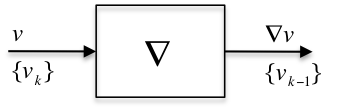
\includegraphics{pictures/blockd.png}}\end{center}
\end{slide}

%----------------------------------------------------------------
% The end of notes
% ----------------------------------------------------------------
\endinput

% Local Variables:
% TeX-master: "lecture02"
% End:
